\documentclass[12pt,a4paper,openright,twoside]{report}

\usepackage[italian]{babel}
\usepackage{newlfont}
\usepackage{parskip}
\usepackage[utf8]{inputenc}
\usepackage{fancyhdr}
\usepackage{hyperref}
\usepackage{geometry}
\usepackage{babelbib}

%serve solo per il frontespizio
\textwidth=455pt %\oddsidemargin=0pt

% Direttive fancyhdr, si può fare riferimento al layout:
% {lhead}   {chead}   {rhead}
%        <Page content>
% {lfoot}   {cfoot}   {rfoot}

\pagestyle{fancy}%\addtolength{\headwidth}{20pt}
\renewcommand{\chaptermark}[1]{\markboth{\thechapter.\ #1}{}}
\renewcommand{\sectionmark}[1]{\markright{\thesection \ #1}{}}
\rhead[\fancyplain{}{\bfseries\leftmark}]{\fancyplain{}{\bfseries\thepage}}
\lhead{\leftmark}
\rhead{\thepage}
\cfoot{}

\linespread{1.2}

\begin{document}

%frontespizio
% Frontespizio reperito da: https://corsi.unibo.it/magistrale/ScienzeInternet/tesi-in-latex
% e liberamente modificato da Guglielmo Palaferri


%\documentclass[12pt,a4paper]{report}
%\usepackage[italian]{babel}
%\usepackage{newlfont}
%
%\begin{document}



\begin{titlepage}
\begin{center}
    

{{\Large{\textsc{Alma Mater Studiorum $\cdot$ Universit\`a di
Bologna}}}} \rule[0.1cm]{15.8cm}{0.1mm}
\rule[0.5cm]{15.8cm}{0.6mm}
{\small{\bf SCUOLA DI INGEGNERIA E ARCHITETTURA\\
Corso di Laurea in Ingegneria Informatica }}
\end{center}
\vspace{35mm}
\begin{center}
{\LARGE{\bf Porting di un algoritmo per la stima del flusso ottico su smartphone Android}}\\
\end{center}
\vspace{50mm}
\par
\noindent
\begin{minipage}[t]{0.47\textwidth}
{\large{\bf Relatore:\\
Prof.\\
STEFANO MATTOCCIA}}
\end{minipage}
\hfill
\begin{minipage}[t]{0.47\textwidth}\raggedleft
{\large{\bf Candidato:\\
GUGLIELMO PALAFERRI}}
\end{minipage}
\vspace{20mm}
\begin{center}
{\large{\bf Appello II\\%inserire il numero della sessione in cui ci si laurea
Anno Accademico 2020-2021}}%inserire l'anno accademico a cui si è iscritti
\end{center}
\end{titlepage}

%\end{document}

\newpage
\clearpage{\pagestyle{empty}\cleardoublepage}

\pagenumbering{roman} %numerazione romana per le pagine di prefazione

%il textwidth=455pt serve per il frontespizio, è troppo grande per il testo
\newgeometry{textwidth=426pt}

\chapter{Introduzione}
%\addcontentsline{toc}{chapter}{Introduzione}
%\lhead{INTRODUZIONE}

Il monitoraggio costante della velocità di fiumi e correnti d'acqua può assumere notevole importanza sia nello studio di 
fenomeni idrologici puramente naturali, sia nella progettazione di opere ingegneristiche strettamente legate ad un 
particolare flusso d'acqua. Ad esempio, può aiutare ad analizzare e rilevare fenomeni come le inondazioni (specie gli 
avvenimenti improvvisi, che destano particolare attenzione), così come anche il trasporto di sedimenti o 
l'erosione delle rocce.

Come evidenziato in \cite{rs10122010}, molte delle tecniche tradizionali utilizzate per l'osservazione di un flusso idrico, tuttavia, non garantiscono 
grande efficienza e presentano costi elevati: spesso è richiesta la presenza di personale specializzato per la 
manutenzione di dispositivi complessi.\\ %citazione a paper remote sensing
Una soluzione che preveda invece l'installazione di apparecchi ottici, e basi quindi il monitoraggio sull'elaborazione di
immagini, può consentire di abbattere notevolmente i costi e di distribuire il sistema di osservazione ottenendo quindi 
maggiore resistenza ai guasti.%inserire immagine di esempio applicazione OTV.

\begin{figure}[h!]
    \begin{center}
        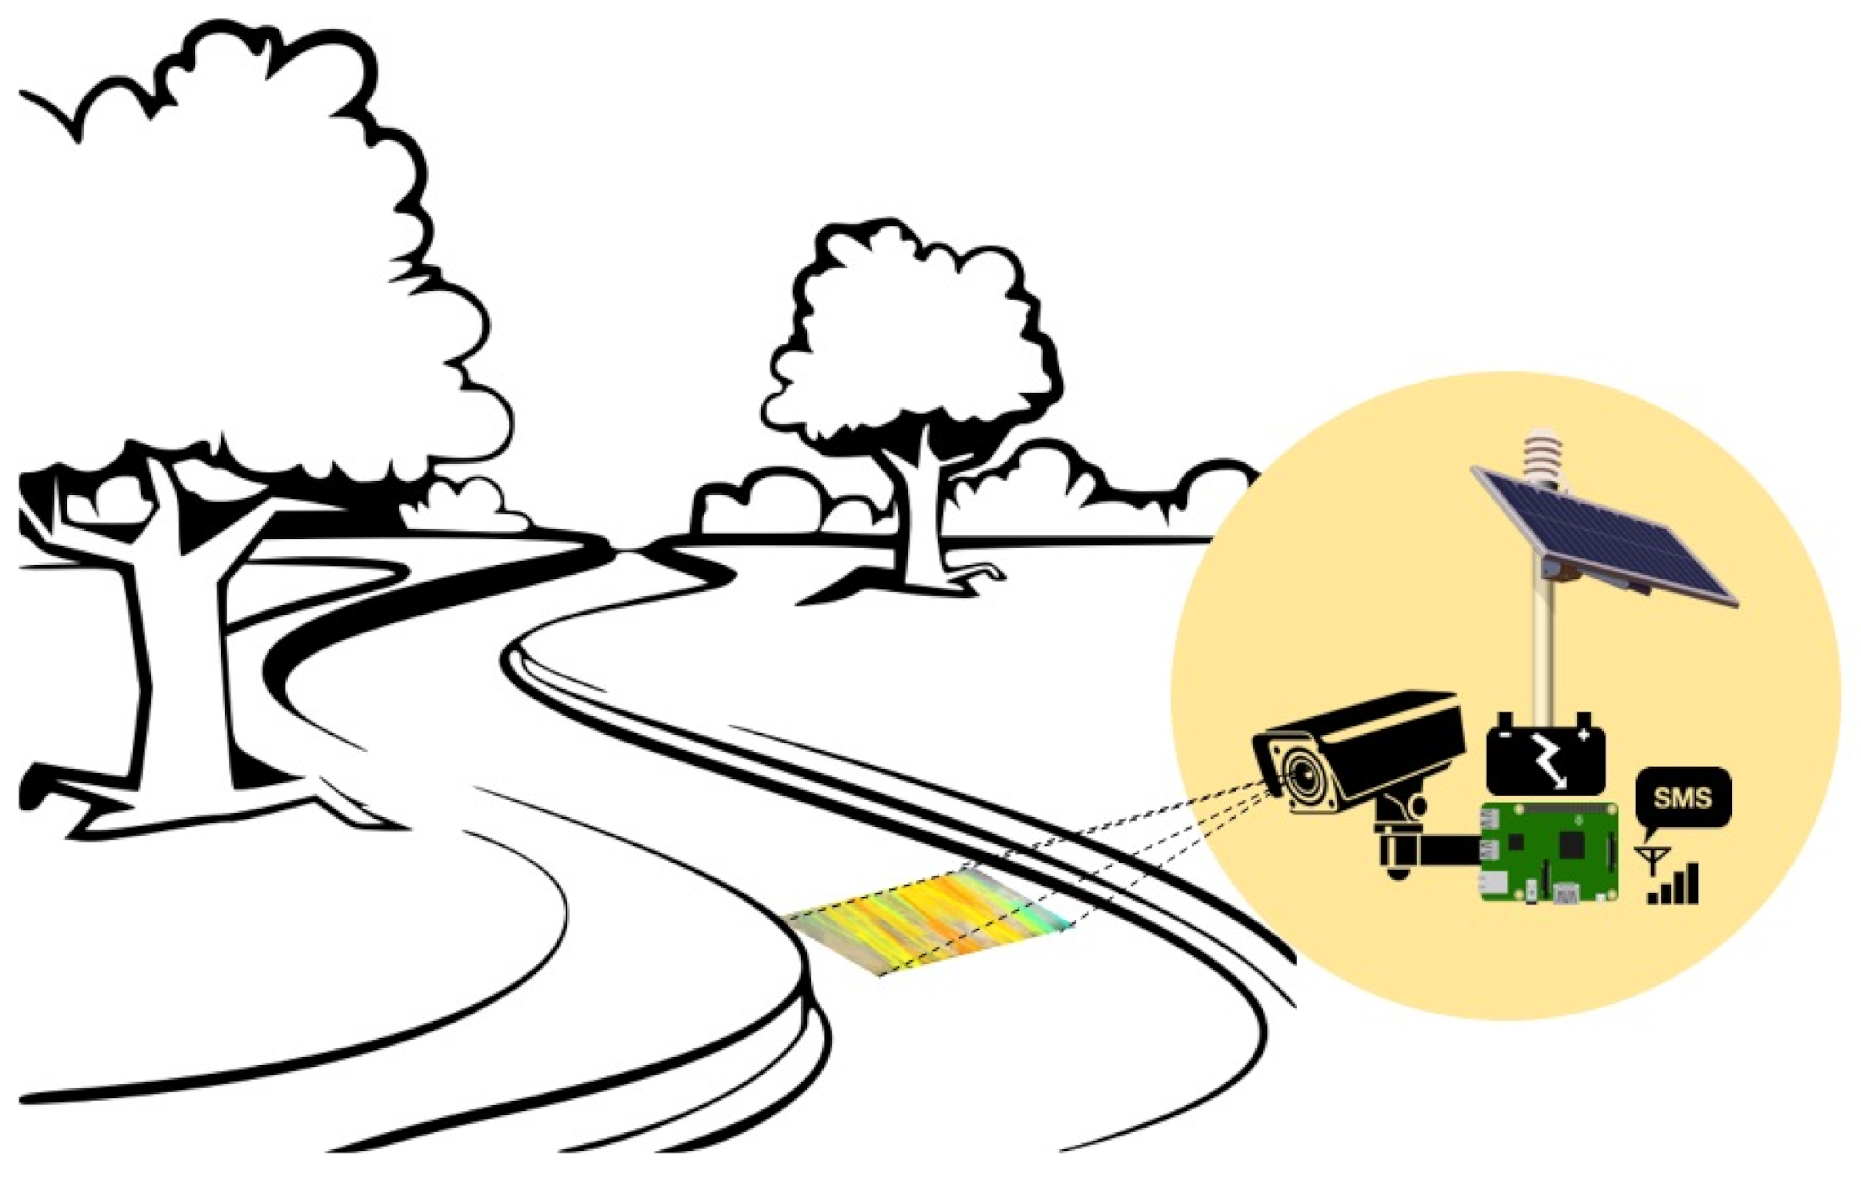
\includegraphics[scale=0.2]{img/otv_real_use.png}
        \caption{Esempio di installazione di un dispositivo embedded basato sull'elaborazione ottica}
    \end{center}
\end{figure}

È proprio questo un caso di utilizzo di \textbf{OTV} (\textit{Optical Tracking Velocimetry}), una tecnica che fa uso di 
particolari algoritmi di computer vision (in particolare l'algoritmo di \textit{Lucas-Kanade}, utilizzato per la stima 
del flusso ottico) per tracciare le traiettorie e le velocità del flusso d'acqua a partire da una serie di immagini. 
Il tracciamento viene svolto grazie al riconoscimento di particelle quali detriti e altri residui e al confronto di fotogrammi 
consecutivi.

Il metodo OTV è pensato per essere applicato a dispositivi di elaborazione a basso costo e di dimensioni contenute: questi
sarebbero posizionati lungo corsi d'acqua in aree geografiche remote. I dati poi raccolti da questi dispositivi potranno essere
spediti (tramite meccanismi semplici come l'invio di SMS) ad un sistema di raccolta dati centralizzato.
Va da sé dunque che l'ottimizzazione dei consumi energetici dei dispositivi costituisca un punto cruciale per la 
realizzabilità di un tale sistema di monitoraggio. Questo tema verrà preso in considerazione e rappresenta uno dei punti
principali degli studi finora condotti sull'argomento.

\begin{figure}[h!]
    \begin{center}
        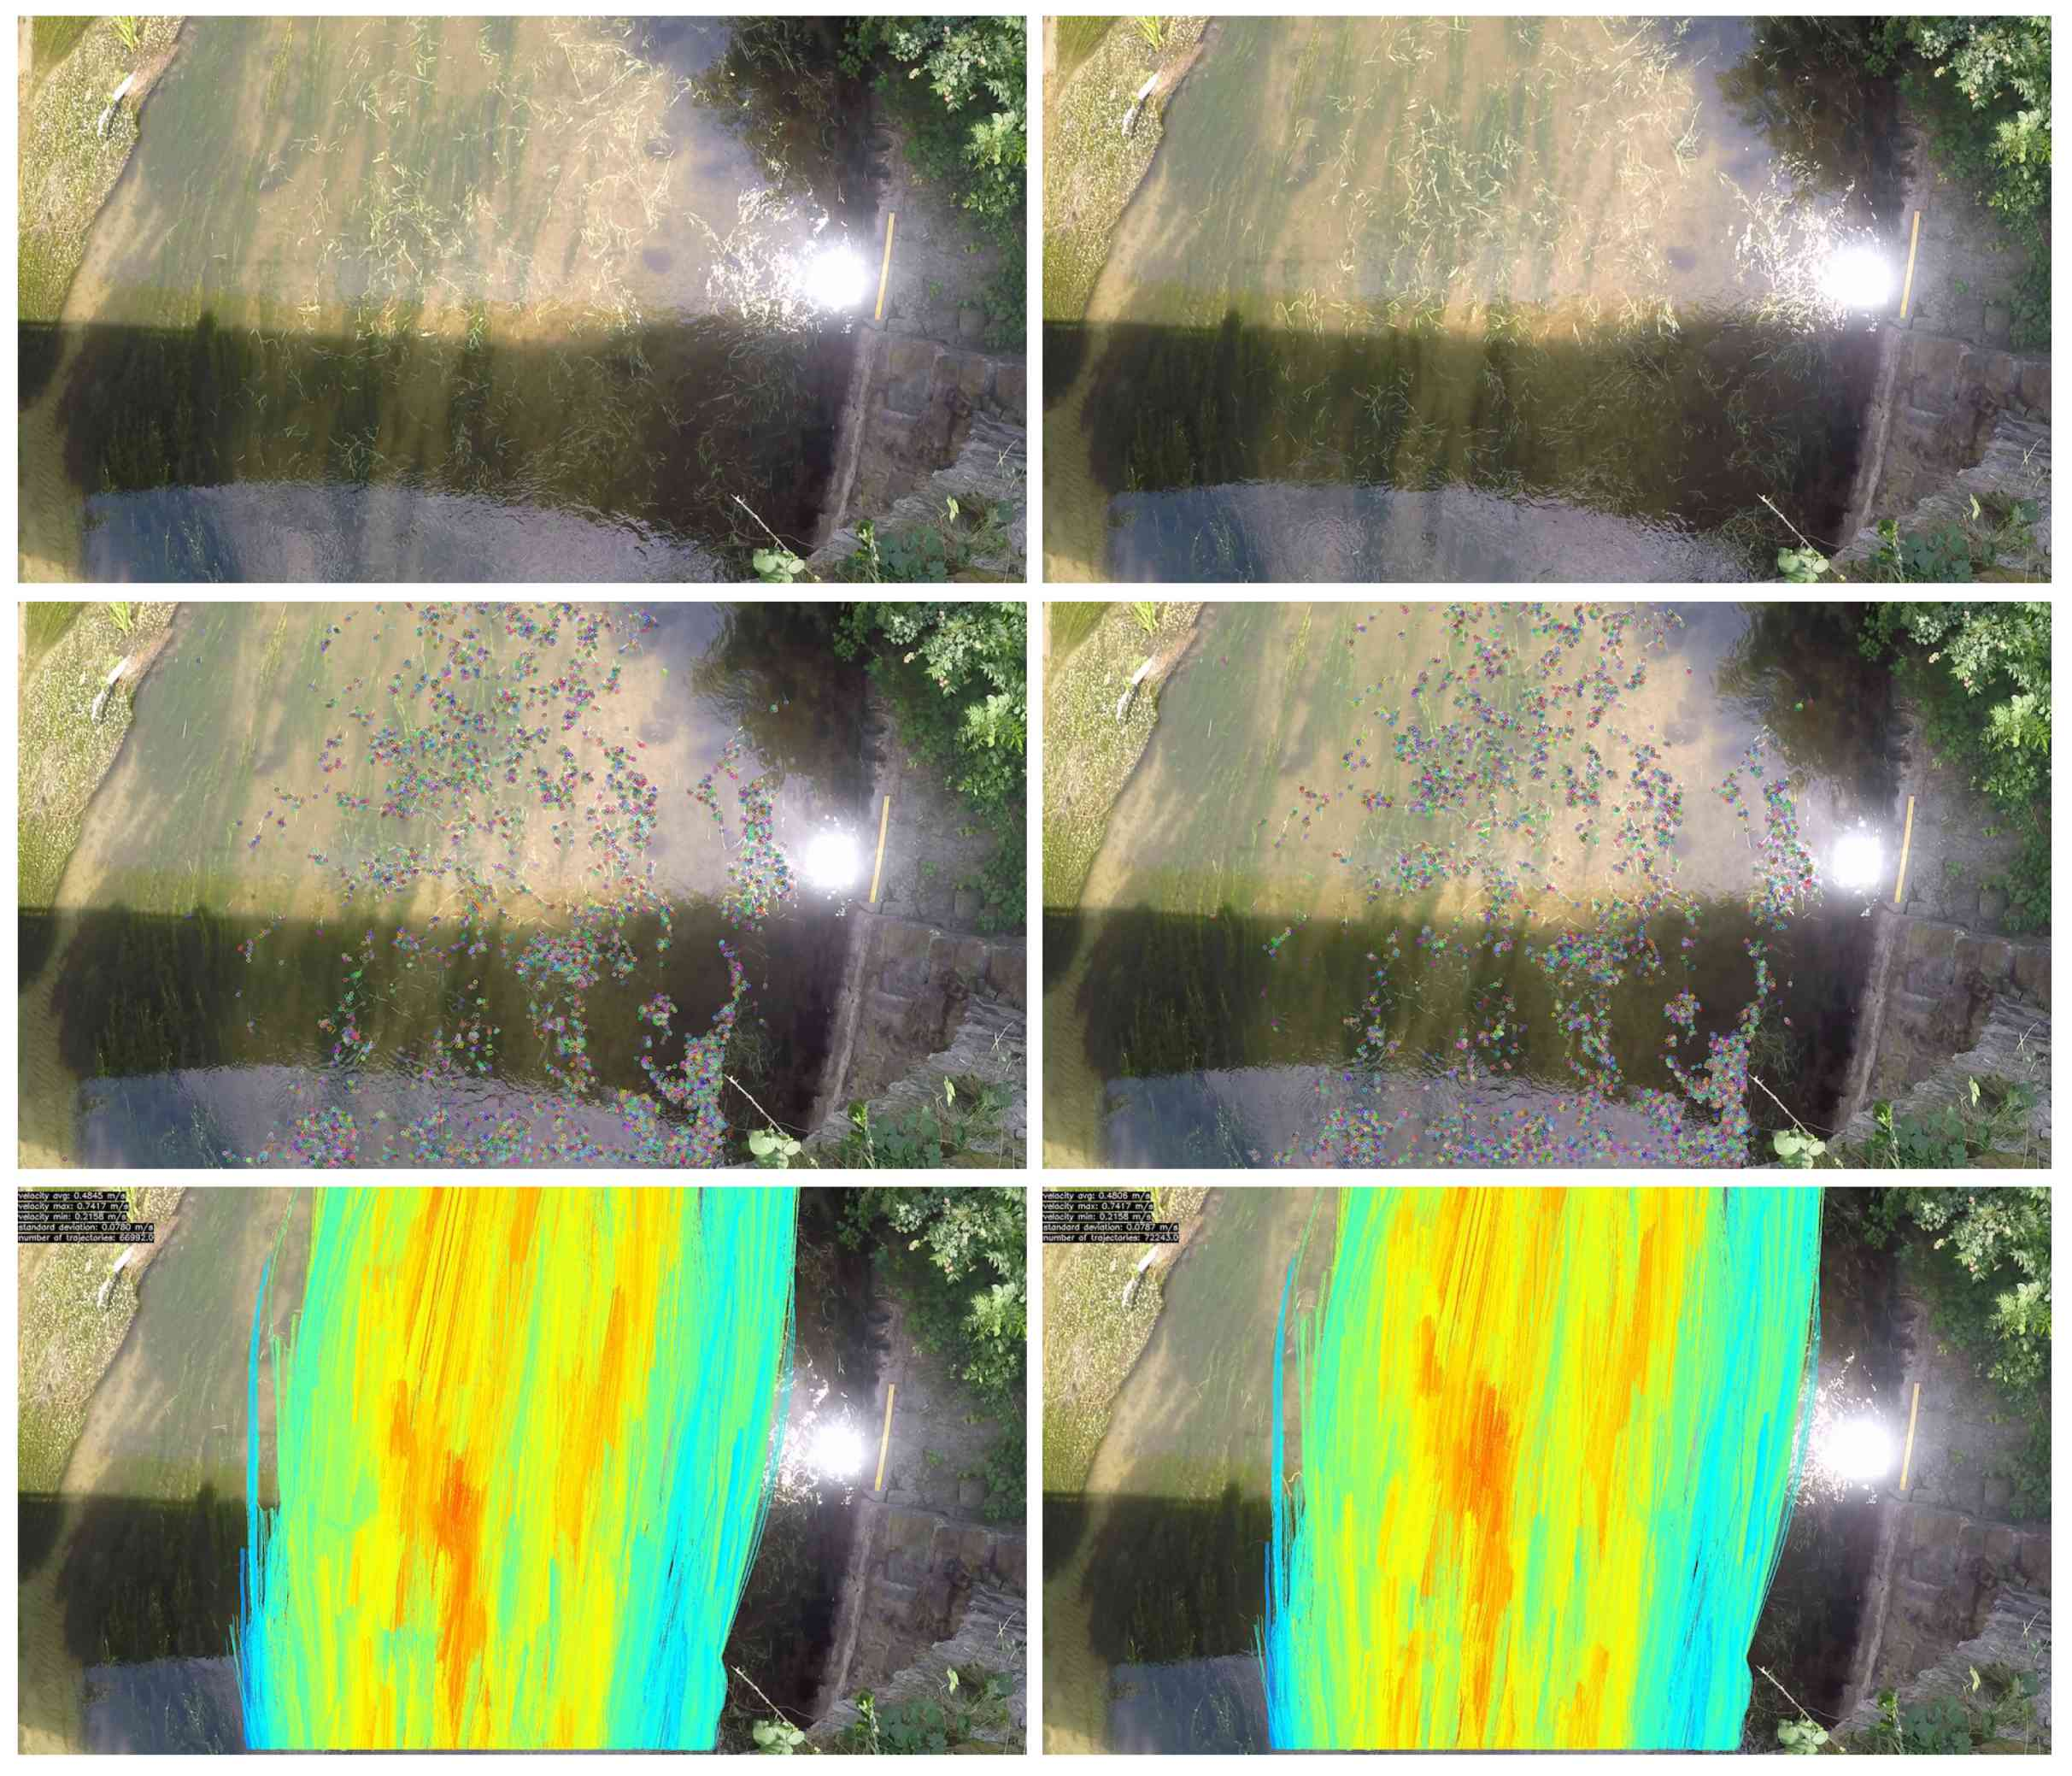
\includegraphics[scale=0.13]{img/sequenze_video_otv.png}
        \caption{Sequenze video ottenute con OTV: le linee tracciate rappresentano le traiettorie riconosciute, colorazioni
        più calde indicano velocità maggiori}
    \end{center}
\end{figure}

L'algoritmo è stato inizialmente testato su dispositivi della famiglia \textit{Raspberry}, per via delle loro dimensioni molto
contenute e in generale per le funzionalità da essi offerte, molto coerenti con i requisiti del progetto. Le analisi \cite{app11157027} 
hanno riportato ottimi risultati dal punto di vista dei consumi energetici in particolare dei modelli Raspberry Pi 3B e 4. 

Altri dispositivi con buone potenzialità e con un profilo che si presti bene al contesto di utilizzo sono gli \textbf{smartphone},
con particolare riferimento a quelli basati su sistema operativo \textbf{Android}. L'utilizzo di tali dispositivi richiede ovviamente
una seppur minima quantità di modifiche rispetto al deployment effettuato su Raspberry, ed è proprio questo il tema centrale
del seguente documento.

Nei prossimi capitoli si procede quindi --- dopo aver introdotto qualche informazione necessaria su OTV --- a descrivere 
la realizzazione di un'applicazione per smartphone Android che adatti l'implementazione in C++ di OTV (disponibile su GitHub al link 
\cite{otvgit}) e i risultati in termini di prestazioni e consumi energetici che ne sono conseguiti.




\clearpage{\pagestyle{empty}\cleardoublepage}

\tableofcontents
%\rhead[\fancyplain{}{\bfseries\leftmark}]{\fancyplain{}{\bfseries\thepage}}
%\lhead[\fancyplain{}{\bfseries\thepage}]{\fancyplain{}{\bfseries
%INDICE}}
\clearpage{\pagestyle{empty}\cleardoublepage}

\lhead[\fancyplain{}{\bfseries\thepage}]{\fancyplain{}{\bfseries\rightmark}}
\pagenumbering{arabic} %numerazione araba per il contenuto effettivo

%++++++++++++

\chapter{Utilizzo di OTV}
\section{Prima sezione}




\clearpage{\pagestyle{empty}\cleardoublepage}

%===========

%\chapter{Processo di sviluppo}
%\section{Prima sezione}




%\clearpage{\pagestyle{empty}\cleardoublepage}

%===========

%\chapter{Testing e misurazioni}
%\section{Prima sezione}




%\clearpage{\pagestyle{empty}\cleardoublepage}

%===========

%\chapter*{Conclusioni}




%\clearpage{\pagestyle{empty}\cleardoublepage}


% --------------- Fine contenuto, inizio bibliografia ---------------

\bibliographystyle{abbrv}
\bibliography{refs}

%\begin{thebibliography}{90}             %crea l'ambiente bibliografia

    %\rhead[\fancyplain{}{\bfseries \leftmark}]{\fancyplain{}{\bfseries
    %\thepage}}
    %\addcontentsline{toc}{chapter}{Bibliografia}

    %\bibitem{K1} .
    %\bibitem{K2} Secondo oggetto bibliografia.
    %\bibitem{K3} Terzo oggetto bibliografia.
    %\bibitem{K4} Quarto oggetto bibliografia.

%\end{thebibliography}

\end{document}